	\documentclass[10pt,oneside]{CBFT_book}
	
	% Algunos paquetes
	
	\usepackage{amssymb}
	\usepackage{amsmath}
	\usepackage{graphicx}
	\usepackage{libertine}
	\usepackage[bold-style=TeX]{unicode-math}
	\usepackage{lipsum}

	\usepackage[numbers]{natbib}
	\setcitestyle{square}


	\usepackage{polyglossia}
	\setdefaultlanguage{spanish}

	\usepackage{CBFT.estilo} % Cargo la hoja de estilo
	

	% Tipografías
	% \setromanfont[Mapping=tex-text]{Linux Libertine O}
	% \setsansfont[Mapping=tex-text]{DejaVu Sans}
	% \setmonofont[Mapping=tex-text]{DejaVu Sans Mono}

	%===================================================================
	%	DOCUMENTO PROPIAMENTE DICHO
	%===================================================================

% \title{CBFT Mecánica clásica}
% \author{Mecánica lagrangiana}
% \date{\today}

\begin{document}
% \maketitle
% \tableofcontents
\chapter{Mecánica newtoniana}

% =================================================================================================
\section{Momento angular}
% =================================================================================================

\[
	\vb{L} = \vb{r} \times \vb{p}
\]
\begin{figure}[hbt]
	\begin{center}
	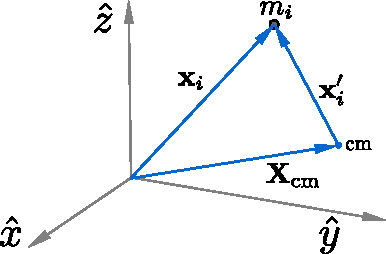
\includegraphics[width=0.3\textwidth]{images/fig_mc_angularmom.pdf}	
	\end{center}
	\caption{}
\end{figure} 
\[
	\vb{r}_i = \vb{R} + \vb{r}_i' \qquad \vb{v}_i = \vb{V} + \vb{v}_i'
\]
\[
	\vb{L}^T_O = \sum_i \vb{r}_i \times \vb{p}_i = \sum_i (\vb{R} + \vb{r}_i') \times m_i (\vb{V} + \vb{v}_i')
\]
\[
	\vb{L}^T_O = \sum_i ( \vb{R} \times m_i \vb{V}  + \vb{R} \times m_i \vb{v}_i'
	+ \vb{r}_i' \times m_i \vb{V} 	+ \vb{r}_i' \times m_i \vb{v}_i' )
\]
pero si recordamos que se cumplen 
\[
	\vb{R} = \sum_i \frac{m_i \vb{r}_i}{M}
\]
\[
	M\vb{R} = \sum_i m_i (\vb{R} + \vb{r}_i') = \sum_i m_i \vb{R} + \sum_i m_i \vb{r}_i'
\]
\[
	M\vb{R} = M \vb{R} + \sum_i m_i \vb{r}_i' \quad \Longrightarrow 0 = \sum_i m_i \vb{r}_i'
\]
podemos volver a las ecuaciones anteriores para poner
\[
	\vb{L}^T_O = \vb{R} \times M \vb{V}  + \vb{R} \times \frac{d}{dt}\left( m_i \vb{r}_i' \right)
	+ \left( \sum_i m_i \vb{r}_i' \right) \times \vb{V} + \sum_i \vb{r}_i' \times m_i \vb{v}_i'
\]
\[
	\vb{L}^T_O = \vb{R} \times M \vb{V}  + \sum_i \vb{r}_i' \times m_i \vb{v}_i'
\]
\[
	\vb{L}^T_O = \vb{L}^{cm} + \vb{L}^{sist}_{cm}
\]
siendo el primer término del lado derecho el momento angular orbital y el segundo el momento angular
de spin.

Con respecto a la conservacion del momento angular, se tendrá
\[
	\dtot{\vb{L}_O}{t} = \sum \vb{\tau}_O
\]
que se puede ver como suma del torque de fuerzas externas y de fuerzas internas. En el primer caso,
los torques externos sumarán cero si las fuerzas externas son nulas o centrales.
En el segundo caso los torques internos son nulos si vale el principio de acción y reacción fuerte;
es decir si
\[
	\vb{r}_i - \vb{r}_j \parallel F_{ij}.
\]

% =================================================================================================
\section{Trabajo y energía}
% =================================================================================================

\[
	T_2 - T_1 = W_{1 \to 2} = U_1 - U_2 
\]
donde la primera igualdad vale siempre y la segunda se da si se puede escribir la fuerza como el
gradiente de un potencial, i.e.
\[
	\vb{F} = - \nabla U
\]
y entonces se conserva la energía
\[
	T_2 + U_2 = T_1 + U_1
\]

Sólo las componentes tangenciales de la fuerza producen trabajo.
\begin{figure}[hbt]
	\begin{center}
	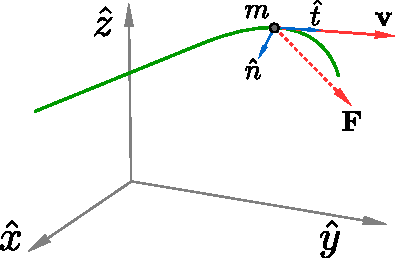
\includegraphics[width=0.3\textwidth]{images/fig_mc_workenergy.pdf}	
	\end{center}
	\caption{}
\end{figure} 

\[
	m \dtot{\vb{v}}{t} = \vb{F}
\]
entonces
\[
	m \dtot{v}{t} = F_t \qquad m \frac{v^2}{\rho} = F_n
\]
y haciendo un cambio de variable a desplazamiento $s$
\[
	m dv \dtot{s}{t} = F_t ds
\]
\[
	m \int v dv = \int F_t ds = \int \vb{F} \cdot d\vb{s}
\]
\[
	\left. \frac{1}{2} m v^2 \right|_i^f = W_{i \to f}
\]
siendo este resultado el llamado {\it teorema de las fuerzas vivas}. 
Notemos que el versor desplazamiento $d\vb{s}$ {\it camina} por la trayectoria.

\[
	W = W^{ext} + W^{int}
\]
y entonces como el trabajo externo viene de 
\[
	\sum_i^N \int \vb{F}^{ext}_i \cdot d\vb{s}_i
\]
necesito $\vb{F}_i = \vb{F}_i(\vb{r}_i)$ y $\nabla \times \vb{F}_i=0$.
Para el trabajo interno
\[
	W_i^{int} = \int \sum_j^N  \vb{F}_{ij} \cdot d\vb{s}_i
\]
\[
	W^{int} = \sum_i \int \sum_j  \vb{F}_{ij} \cdot d\vb{s}_i
\]
\[
	\frac{1}{2} \sum_i \sum_j \int \vb{F}_{ij} \cdot d\vb{s}_i + \vb{F}_{ji} \cdot d\vb{s}_j =
	\frac{1}{2} \sum_i \sum_j \int \vb{F}_{ij} \cdot \left( d\vb{s}_i - d\vb{s}_j \right)
\]

% =================================================================================================
\section{Definiciones}
% =================================================================================================

El número de grados de libertad es el número de coordenadas independientes para resolver el problema.
Las fuerzas de vínculo $F^v$ se {\it acomodan} en todo momento para satisfacer las ligaduras.
Entonces las $\vb{F}^v$ son perpendiculares a los desplazamientos compatibles con los vínculos de
manera que 
\[
	W_{F^v} = 0
\]
\begin{figure}[hbt]
	\begin{center}
	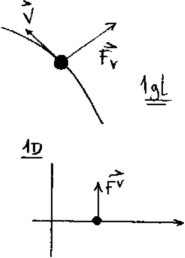
\includegraphics[width=0.3\textwidth]{images/fig_mc_vinculos1.pdf}	 
	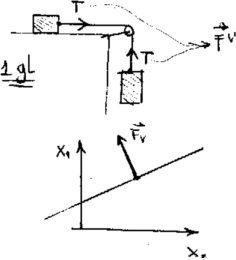
\includegraphics[width=0.3\textwidth]{images/fig_mc_vinculos2.pdf}
	\end{center}
	\caption{}
\end{figure} 

Los vínculos se clasifican en
\[
\textrm{holónomos} 
\begin{Bmatrix}
 f(r_i,t) = 0 \qquad \textrm{reónomos} \\
\; f(r_i) = 0 \qquad \textrm{esclerónomos} \;\\
\end{Bmatrix} 
\]
los cuales cumplen que  $W_{virtual}^{F^v}=0$, y
\[
\textrm{no holónomos} 
\begin{Bmatrix}
 f(r_i,t) \geq 0  \\
 f(r_i) \geq cte. \quad f(\dot{r}_i) = 0  \; \\
\end{Bmatrix}
\]
los cuales no cumplen, en general, que $\vb{F}^v$ perpendicular al desplazamiento posible.
\begin{figure}[hbt]
	\begin{center}
	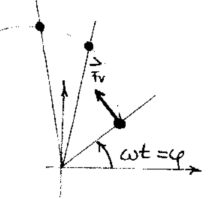
\includegraphics[width=0.3\textwidth]{images/fig_mc_vinculos3.pdf}	
	\end{center}
	\caption{}
\end{figure} 
donde un desplazamiento virtual es un desplazamiento a $t_0$ fijo compatible con los vínculos,
mientras que un desplazamiento real es un desplazamiento en $\delta t$ durante el cual varían
fuerzas y ligaduras.

A tiempo fijo el desplazamiento es en $\hat{r} \perp \vb{F}^v$.

\[
	f(x_i,t) = cte. \Longrightarrow \sum_i^N \dpar{f}{x_i} \delta x_i + \dpar{f}{t} \delta t = 0 
\]
o bien
\[
	\nabla f \cdot \vb{\delta r} = 0
\]
% Como ejemplo citamos \cite{einstein}.
% O bien \cite{example}.
% Tal vez \citep{Aspnes:1973}

% ============================================================================

% \bibliographystyle{CBFT-apa-good} % (uses file "apa-good.bst")
% \bibliography{CBFT.Referencias} % La base de datos bibliográfica


\end{document}
